\documentclass[letter, 10pts]{article}
\usepackage[monocolor]{../math232/ahsansabit}
\usepackage[]{float}
\usepackage{tikz}
\usepackage{tikz-3dplot}
\usepackage[outline]{contour} % glow around text
\usepackage{xcolor}
\usepackage{pdfpages}
\usepackage{physics}
\usepackage{multicol}
\title{Intermediate Electrodynamics : : Homework 04}
\author{Ahmed Saad Sabit, Rice University}
\date{\today}
\newcommand{\hb}{\hbar}
\newcommand{\U}{\uparrow}
\newcommand{\D}{\downarrow}
\usepackage[]{braket}
\begin{document}
\maketitle


\section*{Problem 1}
\subsection*{Solving the general equation for this specific case}
As explained in the problem hint, we can write for $s < R$ (as $\ln s$ and $s^{- k }$ cannot be solved for $s = 0$ which is the center of cylinder)
\[
V = \sum s^{k} (a_k  \cos k \phi + b_k \sin k \phi ) 
\] 

Similarly, for $s > R$ we need solutions that behave properly for $s \to  \infty$
\[
V = \sum s^{-k} (c_k \cos k \phi + d_k \sin k \phi) 
\]
Now according to the problem hint we can use 
\[
\frac{\partial V}{\partial s} (R+) - \frac{\partial V}{\partial s} (R-) =  - \frac{\sigma}{\epsilon_0}
\] 
For this we need to isolate the equations of the potential above and below the surface. We do this in the following analysis. 

Potential is continuous so $V_{(s<R)}(R)  = V_{(s>R)}(R)$. This helps us solve for each term of the summation
\[
\sum R^{k} (a_k  \cos k \phi + b_k \sin k \phi ) 
= \sum R^{-k} (c_k \cos k \phi + d_k \sin k \phi) 
\] Considering each term 
\[
 R^{2k} (a_k  \cos k \phi + b_k \sin k \phi ) 
= (c_k \cos k \phi + d_k \sin k \phi) 
\] 
Equality 
\[
c_k = R^{2k} a_k
\] 
\[
d_k = R^{2k} b_k
\] 
Now we can use this information in our old formula 
\[
\frac{\partial V}{\partial s} (R+) - \frac{\partial V}{\partial s} (R-) =  - \frac{\sigma}{\epsilon_0}
\] What we get is 
\[
\sum 
2k R^{k-1} (a_k \cos k \phi + b_k \sin k \phi) = - \frac{\sigma}{\epsilon_0}
\] 
But BEWARE! The sign of $\sigma$ changes. So, for $0<\phi < \pi$ what we get
\[ \sum 
2k R^{k-1} (a_k \cos k \phi + b_k \sin k \phi) = \frac{\sigma_0}{\epsilon_0}
\] 
And for $0 < \phi < 2 \pi $ we get
\[ \sum 
2k R^{k-1} (a_k \cos k \phi + b_k \sin k \phi) = - \frac{\sigma_0}{\epsilon_0}
\] 

\subsection*{Solving for the coefficients} 
Using the methods of PHYS 311 we can isolate each coefficients. Because $a_k$ is paired with a $\cos k \phi$ we can do the following integral to find $a_k$ 
\[ \int_0^{2 \pi } \left(
\sum
2k R^{k-1} (a_k \cos k \phi + b_k \sin k \phi) 
\right) (\cos p \phi) \, \mathrm{d} \phi
\] 
This whole integral cannot be done right away in the right hand side where depending on $\phi$ we have $\sigma \to  \sigma_0 \to  - \sigma_0$, but taking care of that and solving integral on the left
\[
 2 \pi p R^{p - 1} a_p = \frac{\sigma_0}{\epsilon_0} 
 \left(
\int_{0}^{\pi } \cos p \phi \, \mathrm{d} \phi - 
\int_{\pi }^{2 \pi } \cos p \phi \, \mathrm{d}  \phi  
 \right) = 0
\] 
This implies 
\[
	a_p = 0 \tag{for all $p$ }
\] 

Very similar we slap a $\sin p \phi$ in both sides and take the exact same integral and get
\[
2 \pi p R^{p -1} b_p = 
\frac{\sigma_0}{\epsilon_0} 
\left(
\int_{0}^{ \pi } \sin p \phi 
- 
\int_{\pi }^{2 \pi }  \sin p \phi 
\right)
\]
I use an integral table and integral-calculator.com help to compute what is above and get, 
\[
= \frac{\sigma_0}{p \epsilon_0} (2  - 2 \cos p \pi)
\]
Because $p$ is integer, if it is even then $ = 0$ and $= 4 \sigma_0 / p \epsilon_0$ otherwise. 
\[
2  \pi p R^{p -1} b_p = 
\begin{cases}
	0 &p \text{ is even} \\ 
	4 \sigma_0 / p \epsilon_0 & p \text{ is odd}
\end{cases} \implies 
b_p = 
\begin{cases}
	0 &p \text{ is even} \\ 
	2 \sigma_0 / \pi \epsilon_0 p^2 R^{p  - 1 } & p \text{ is odd}
\end{cases} 
\] 
We ended up getting very nice solution where for inside $s < R$
\[\boxed{
V = \sum_{}^{} F(s, \phi, a_i, b_j) \implies \frac{2 \sigma_0 R}{\epsilon_0 \pi } 
\sum_{p \in \text{odd}} \frac{(s / R)^{k} \sin(p \phi)}{p^2}
}\] 
For outside
\[
	\boxed{
V = \sum_{}^{} F(s, \phi, a_i, b_j) \implies \frac{2 \sigma_0 R}{\epsilon_0 \pi } 
\sum_{p \in \text{odd}} \frac{(R / s)^{k} \sin(p \phi)}{p^2}
}\] 



\section*{Problem 2} 
\subsection*{(a)}
The paper calculation is attached for further information. 

We notice that 
\[
	V = \frac{1}{4 \pi \epsilon_0} 
	\sum_{n=0}^{\infty} \frac{1}{r^{n + 1}}
	\int_{-\infty}^{\infty} (r')^{n} \mathcal P_1(\cos \alpha) \rho(\vec{r}') \, \mathrm{d} \tau'  
\] 
\[
	V = \frac{1}{4 \pi \epsilon_0} 
	\sum_{n=0}^{\infty} \frac{1}{r^{n + 1}}
	\int_{-\infty}^{\infty} (r')^{n} \mathcal P_1(\cos \alpha) \delta(x') \delta(y') \lambda(z) \, \mathrm{d} x' \mathrm{d} y' \mathrm{d} z'
\] 
So a monopole solution would look like
\[
V = \frac{1}{4 \pi \epsilon_0}
\frac{1}{r} 
\int_{\infty}^{} \lambda \mathrm{d} z 
\] 
In the paper calculation we find that $\lambda = k \cos \pi z / 2 a$ gives us the first leading term 
\[
\boxed{
\frac{1}{4 \pi \epsilon_0} \left(\frac{1}{r}\right)\left(\frac{4 a k }{\pi}\right) = \frac{ak}{\pi ^2 \epsilon_0 r}
}
\] 

\subsection*{(b)} 
Just by analogy to wavefunction in a box solution we can easily see that monopole term for this case $\lambda = k \sin ( \pi  z / a)$ is zero as $ \int \lambda(z) \mathrm{d} z$ is zero. 

To solve for $\cos \alpha$ 
\[
\vec{r} \cdot  \vec{r}' = r r' \cos \alpha \implies (x,y,z)\cdot (0,0,z') = z z' \cos (\alpha) \implies \frac{z}{r} = \cos \alpha 
\] 
Computing the next term (dipole) (explicitly calculated on paper)
\[
\int_{-\infty}^{\infty} 
\sqrt{x'^2 + y'^2 + z'^2} \delta(x) \delta(y) \lambda(z) \, \mathrm{d} x' \mathrm{d} y' \mathrm{d} z'
\cos (\alpha)
\] 
\[ = 
\frac{z}{r} \int_{-a}^{a} k z' \sin ( \pi z' / a  ) \, \mathrm{d} z' = \frac{z}{r} \left(\frac{2 a^2 k}{\pi  }\right)
\] 
We get
\[
\boxed{
\frac{1}{4 \pi \epsilon_0} \frac{1}{r^2} \frac{z}{r} \frac{2 a^2 k }{\pi }
}
\] 
I acknowledge that information about $z$ (or perhaps angle between $\vec{r}$ and $\vec{r}'$) is not explicitly mentioned in the problem. 

\subsection*{(c)} 
Using an integral calculator it shows that for $\lambda = k \cos(\pi z / a)$ both $\int \lambda $ and $\int z \lambda$ are zero. So we calculate the next (quadrupole) term. 

Legendre polynomial for $\cos \alpha$ in this case is $\frac{1}{2} (3 \cos ^2 \alpha - 1)$ where $\cos \alpha = z / r$.

Computing the integral in $-a, a$ we get (using integral-calculator.com)
\[
\int z^2 \cos( \pi z / a) \, \mathrm{d} z = - \frac{4 a^3 k }{\pi ^2}
\] 
Plug everything together using the original multipole expansion we get
\[
\boxed{
\frac{1}{4 \pi \epsilon_0} \left(\frac{1}{2} (3 \cos ^2 \alpha - 1) \right) \left(\frac{1}{r^3}\right) \left(- \frac{4 a^3k }{\pi ^2}\right)
}
\] 
On paper I directly solved everything. 










\section*{Problem 3} 
\begin{figure}[H]
	\centering
	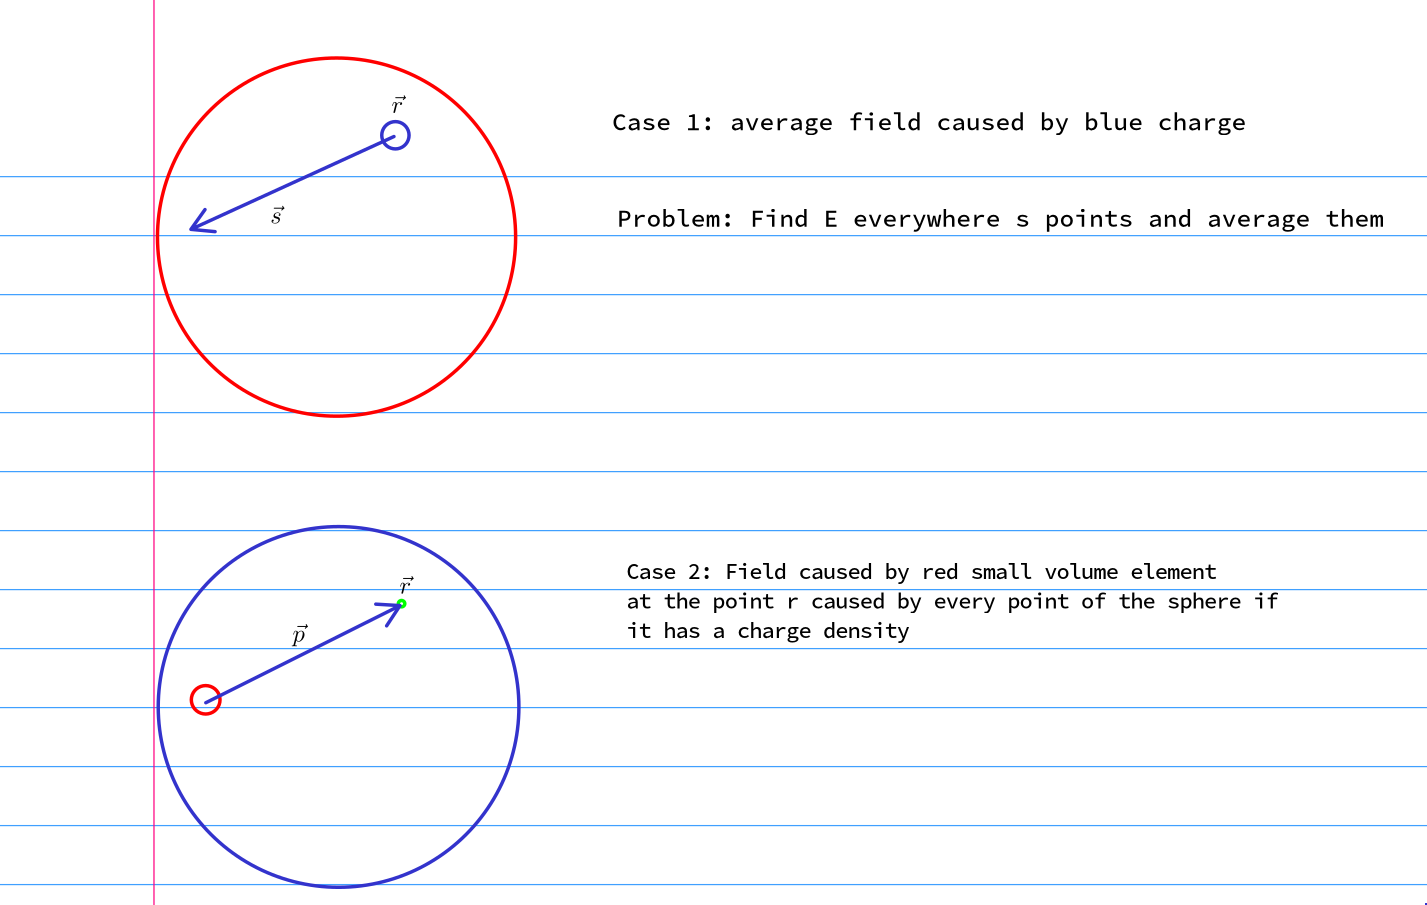
\includegraphics[width=0.8\textwidth]{./fig/4/1.png}
	\caption{./fig/4/1.png}
	\label{fig:-fig-4-1-png}
\end{figure}
\subsection*{(a)}
Use $\vec{s} = \vec{r} - \vec{r}'$ and $\vec{r}'$ be the position of the particle inside the sphere. 
\begin{align*}
\braket{ \vec{E}} &= \frac{1}{4  \pi R^3 / 3} \int_{}^{} \vec{E} \, \mathrm{d} \tau  \\
&= \frac{1}{4 \pi R^3 / 3} \frac{1}{4 \pi \epsilon_0} \int q \frac{\hat{s}}{s ^2} \mathrm{d} \tau \\
&\implies 
\frac{1}{4 \pi \epsilon_0} \int \frac{q}{4 \pi R^3 / 3} \frac{\hat{s}}{s ^2} \mathrm{d} \tau \\
&= \frac{1}{4 \pi \epsilon_0} \int \frac{- q}{4 \pi R^3 / 3} \frac{-\hat{s}}{s ^2} \mathrm{d} \tau \\
&= \frac{1}{4 \pi \epsilon_0} \int \rho \mathrm{d} \tau' \left(\frac{\hat{p}}{p^2}\right) \\
\end{align*}
This last equation exactly replicates the field at $\vec{r}'$ due to uniformly charged sphere with $\rho = - q / \frac{4}{3} \pi R^3$. The negative sign in front of $\vec{s}$ appears because the field lines point opposite to the direction of field ``caused" by a single charge $q$ at $\vec{r}'$.

For ease of thinking we can treat that when $\rho$ is causing the field, it's caused from $\mathrm{d}  \tau$. $\vec{p}$ is the vector from any point of the sphere to designated point of charge. But we just see that it is exactly equal to $\vec{s} = - \vec{p}$.

This, with principal of superposition, will hold for any charge distribution because we solved it for point charge. 


\subsection*{(b)} 
Field from a charge density be $\vec{E}_\rho$ 
\begin{align*}
\vec{E}_\rho &= \frac{1}{3 \epsilon_0} \rho \vec{r}  \\
&= - \frac{q}{4 \pi \epsilon_0} \vec{r}/R^3 \\
&= - \frac{\vec{p}}{4 \pi \epsilon_0 R^3} \\
\end{align*}


\subsection*{(c)} 
\[
E_\rho_1 + E_\rho_2 + \cdots = \sum_{i}^{} E_\rho_i = - \frac{1}{4 \pi \epsilon_0 }  \sum_{i}^{} \frac{\vec{p}_i}{R^3_i}
\] 
Field being averaged $R_i = R$ so 
\[
	\vec{E}_\text{average total} = - \frac{1}{4 \pi \epsilon_0 R^3}  \vec{p}_{\text{net dipole moment}} 
\] 
\subsection*{(d)} 
The field at $\vec{r}$ due to a uniformly charged sphere is 
\[
\vec{E} = \frac{1}{4 \pi \epsilon_0} \frac{q}{r^2} \hat{r} 
\] 
This time $q$ placed at $\vec{r}$ outside the sphere we get
\[
	\vec{E}_{\text{average}} = \frac{1}{4 \pi \epsilon_0} \frac{4 \pi R^3 \rho / 3}{r^2} (-\hat{r}) 
\] 
The negative sign takes care of the fact that the $\vec{r}$ vector has to point inwards for the charge to center. 

But these are technically the same (as shown in (a)). So, the average field due to the point outside is exactly equal to the field produced in the center. Now by adding up each individual point charges we can easily state that this will hold for ANY charge distribution outside of the sphere. 






\section*{Problem 4} 
\subsection*{(a)} 
\begin{align*}
\sigma_B &= \vec{P} \cdot \vec{n} 
\\
&= (k \vec{r}) \cdot  \vec{n}  \\
&= kr \\
\end{align*} 
At the surface the charge is $\sigma_B = k R$. Total charge at the surface, 
\[
Q_\text{surface} = 4 \pi R^3
\] 
\begin{align*}
\rho_B &= - \nabla \cdot  \vec{P} \\
&= -\frac{1}{r^2} \frac{\partial }{\partial r}(r^2 k r)  \\
&= -\frac{1}{r^2} \frac{\partial}{\partial r}(r^3 k)  \\
&= -\frac{k}{r^2} (3 r^2 )  \\
&= -3k \\
\end{align*}
Total charge in the volume is 
\[
Q_\text{volume} = \frac{4}{3} \pi R^3 (- 3 k) = - 4 \pi R^3 
\] 

\textbf{Answers:}
Surface charge density \[
\boxed{
\sigma_B = kR
}
\] 
Volume charge density 
\[
\boxed{
\rho_B = - 3k
}
\] 

\subsection*{(b)} 
For the homogeneous charge distribution inside the surface, hence using Gauss's law we know that the Electric field is just going to be 
\[
	E_r (4 \pi r^2) = (-3k) (4 \pi r^3 / 3\epsilon_0) 
	\implies 
	E_r = - \frac{k}{\epsilon_0}\tag{$r < R$}
\] 

Outside, using Gauss's law
\[
	E_r (4 \pi \mathrm{r}   ) = \frac{Q_\text{surface} + Q_\text{volume} }{\epsilon_0} = 0   
	\tag{$\mathrm{r} > R $}
\]  
The field outside the ball is zero. 

\textbf{Answers:} Electric Field \[
\boxed{E_r =
\begin{cases}
 - k / \epsilon_0 & r < R\\
	 0 & r > R 
\end{cases}} 
\] 




\section*{Problem 5} 
The uniform polarization along $\vec{P} = P \hat{z}$. 
Bound charge 
\[
\rho_B = - \nabla \cdot  \vec{P} = \frac{\mathrm{d} P}{\mathrm{d}z } = 0
\] 
Surface charge (on flat ends) because curved surface would be zero. Top face
\[
\sigma^{\text{top}}_B = \vec{P} \cdot \hat{n} = P
\]
Bottom face
\[
\sigma^{\text{lower}}_B = \vec{P} \cdot  \hat{n} = -P 
\] 
HAND-DRAWN DIAGRAM HAS BEEN ATTACHED AT THE END (BEGINNING).
















\section*{Problem 6} 
Compute the total charge
\[
	Q = \int \mathrm{d} q_{\text{volume}}  + \int \mathrm{d} q_{\text{surface}} 
\]
\begin{align*}
Q &= 
\int \mathrm{d} V (\rho_b) + 
\int \mathrm{d} A (\sigma_b) \\
  &=
- \int \mathrm{d} V (\nabla \cdot \vec{P}) + 
\int \mathrm{d} A (\vec{P} \cdot \vec{n})\\
&= -  \int \mathrm{d} \vec{S} \cdot  \vec{P} + 
\int \mathrm{d} A (\vec{P} \cdot \vec{n})\\
&= - \int \mathrm{d} A  \vec{P} \cdot \hat{n} + 
\int \mathrm{d} A (\vec{P} \cdot \vec{n})\\ 
&= 0 \\
\end{align*}

\end{document}
